\newcommand{\svcourse}{CST Part IA: Software Engineering and Security}
\newcommand{\svnumber}{1}
\newcommand{\svvenue}{Microsoft Teams}
\newcommand{\svdate}{2022-05-11}
\newcommand{\svtime}{15:00}
\newcommand{\svuploadkey}{CBd13xmL7PC1zqhNIoLdTiYUBnxZhzRAtJxv/ytRdM1r7qIfwMsxeVwM/pPcIo8l}

\newcommand{\svrname}{Dr Sam Ainsworth}
\newcommand{\jkfside}{oneside}
\newcommand{\jkfhanded}{yes}

\newcommand{\studentname}{Harry Langford}
\newcommand{\studentemail}{hjel2@cam.ac.uk}


\documentclass[10pt,\jkfside,a4paper]{article}
\usepackage{tikz}
\usetikzlibrary{automata,positioning,arrows}

% DO NOT add \usepackage commands here.  Place any custom commands
% into your SV work files.  Anything in the template directory is
% likely to be overwritten!

\usepackage{fancyhdr}

\usepackage{lastpage}       % ``n of m'' page numbering
\usepackage{lscape}         % Makes landscape easier

\usepackage{verbatim}       % Verbatim blocks
\usepackage{listings}       % Source code listings
\usepackage{graphicx}
\usepackage{float}
\usepackage{epsfig}         % Embed encapsulated postscript
\usepackage{array}          % Array environment
\usepackage{qrcode}         % QR codes
\usepackage{enumitem}       % Required by Tom Johnson's exam question header

\usepackage{hhline}         % Horizontal lines in tables
\usepackage{siunitx}        % Correct spacing of units
\usepackage{amsmath}        % American Mathematical Society
\usepackage{amssymb}        % Maths symbols
\usepackage{amsthm}         % Theorems

\usepackage{ifthen}         % Conditional processing in tex

\usepackage[top=3cm,
            bottom=3cm,
            inner=2cm,
            outer=5cm]{geometry}

% PDF metadata + URL formatting
\usepackage[
            pdfauthor={\studentname},
            pdftitle={\svcourse, SV \svnumber},
            pdfsubject={},
            pdfkeywords={9d2547b00aba40b58fa0378774f72ee6},
            pdfproducer={},
            pdfcreator={},
            hidelinks]{hyperref}

\renewcommand{\headrulewidth}{0.4pt}
\renewcommand{\footrulewidth}{0.4pt}
\fancyheadoffset[LO,LE,RO,RE]{0pt}
\fancyfootoffset[LO,LE,RO,RE]{0pt}
\pagestyle{fancy}
\fancyhead{}
\fancyhead[LO,RE]{{\bfseries \studentname}\\\studentemail}
\fancyhead[RO,LE]{{\bfseries \svcourse, SV~\svnumber}\\\svdate\ \svtime, \svvenue}
\fancyfoot{}
\fancyfoot[LO,RE]{For: \svrname}
\fancyfoot[RO,LE]{\today\hspace{1cm}\thepage\ / \pageref{LastPage}}
\fancyfoot[C]{\qrcode[height=0.8cm]{\svuploadkey}}
\setlength{\headheight}{22.55pt}


\ifthenelse{\equal{\jkfside}{oneside}}{

 \ifthenelse{\equal{\jkfhanded}{left}}{
  % 1. Left-handed marker, one-sided printing or e-marking, use oneside and...
  \evensidemargin=\oddsidemargin
  \oddsidemargin=73pt
  \setlength{\marginparwidth}{111pt}
  \setlength{\marginparsep}{-\marginparsep}
  \addtolength{\marginparsep}{-\textwidth}
  \addtolength{\marginparsep}{-\marginparwidth}
 }{
  % 2. Right-handed marker, one-sided printing or e-marking, use oneside.
  \setlength{\marginparwidth}{111pt}
 }

}{
 % 3. Alternating margins, two-sided printing, use twoside.
}


\setlength{\parindent}{0em}
\addtolength{\parskip}{1ex}

% Exam question headings, labels and sensible layout (courtesy of Tom Johnson)
\setlist{parsep=\parskip, listparindent=\parindent}
\newcommand{\examhead}[3]{\section{#1 Paper #2 Question #3}}
\newenvironment{examquestion}[3]{
\examhead{#1}{#2}{#3}\setlist[enumerate, 1]{label=(\alph*)}\setlist[enumerate, 2]{label=(\roman*)}
\marginpar{\href{https://www.cl.cam.ac.uk/teaching/exams/pastpapers/y#1p#2q#3.pdf}{\qrcode{https://www.cl.cam.ac.uk/teaching/exams/pastpapers/y#1p#2q#3.pdf}}}
\marginpar{\footnotesize \href{https://www.cl.cam.ac.uk/teaching/exams/pastpapers/y#1p#2q#3.pdf}{https://www.cl.cam.ac.uk/\\teaching/exams/pastpapers/\\y#1p#2q#3.pdf}}
}{}


\lstset{language=Python, upquote=true}

\begin{document}

\section{Genome Assembly}

\begin{enumerate}

    \item In the \textit{genome assembly} problem, we augment the previously covered sequencing framework with an additional \textit{reference genome}. In what way does this aid sequencing?

    Most genomes are overwhelmingly similar. This means that when sequencing a new individual, a lot of the work has already been done. Typically, animals of the same species share $\sim 99.9\%$ of their DNA with
    each other. So we can get a reference genome of a ``typical specimen'', find where the differences are and patch over them to create a genome for the new individual much easier than constructing one from
    scratch.

    \item Explain the basic operations supported by the trie data structure and their complexities. Highlight how it can be deployed into the problem of genome assembly in different ways. Your answer should
    provide a discussion of \textit{tries}, \textit{suffix tries} and \textit{suffix arrays}.

    Trie's are a type of lookup data structure which is optimised for the case where keys are prefixes of each other. They support lookups, insertion and deletion. Lookups, insertions and deletions all have time
    complexities $\in \mathcal O(\ell)$ where the length of the key is $\ell$.

    In a trie, you start at the root, move to the node corresponding to the next symbol in the key and repeat until there are no more symbols. If you are at a node, then you are done and the value
    of this node is the value of the lookup.

    A Suffix Trie is a trie which contains all suffixes of a particular piece of text.

    A Suffix Array is an array where the ith element holds the index of first element of the suffix which comes ith when ordered lexicographically. This can be used to do longest prefix match by binary
    searching the array for matches using $\mathit{sequence}[i:]$ as the key. This corresponds to the indices of the symbols in the first row in the intermediate BWT rotation matrix.

    \item Explain how the  methods of the Burrows-Wheeler transform (BWT) and run-length encoding (RLE) can be applied to reducing the storage requirements of large genomes. Prove that your scheme is efficiently
    invertible.

    We start with a genome which isn't particularly amenable to RLE (and path compression in Suffix Tries)\@. The BWT takes this structure and creates a new representation which has a high probability of being
    amenable to RLE\@.

    The BWT is a form of string compression which works particularly well with genome data. Firstly, consider all possible rotations of the string. Then sort the permutations lexicographically. The
    last column of the rotation matrix is the result of the BWT\@. This representation is more likely to have sequences of characters than the original string if the original string has any commonly repeated
    sequences and so can be compressed better using RLE\@.

    BWT has the property that the predecessor to the $i$th occurrence of a symbol $s$ in the last column is at the index corresponding to the $i$th occurrence of that symbol in the first column. Since we know
    the index of the last symbol (EOF), we can inductively use this to find the preceding symbol. This \textit{can} be done in linear time (although my implementation below is quadratic for implementation
    simplicity).

    \item How can one efficiently pattern-match to the string obtained by the above? Your answer should contain a discussion of the properties and construction time complexities of \textit{suffix arrays}.

    \begin{itemize}

        \item Suffix Trie

        We can pattern match in a Suffix Trie by simply looking up the string in the Trie. If we use the BWT'd matrix and path compression then we are likely to have a lower memory complexity.

        \item Suffix Array

        We can pattern match in a Suffix Array by binary searching the array for the prefix desired. This will return a range; where all elements in the range have the same prefix and this is the prefix we
        search for.

    \end{itemize}

    \item Demonstrate all of the techniques outlined in questions 2--4 on the sequence \texttt{CATATATAG\$}.

    I start by demonstrating the BWT on the sequence \texttt{CATATATAG\$}. I then invert it.

    \begin{table}[H]

        \centering

        \begin{tabular}{cccccccccc}
            \texttt C & \texttt A & \texttt T & \texttt A & \texttt T & \texttt A & \texttt T & \texttt A & \texttt G & \$ \\
            \texttt A & \texttt T & \texttt A & \texttt T & \texttt A & \texttt T & \texttt A & \texttt G & \$ & \texttt C \\
            \texttt T & \texttt A & \texttt T & \texttt A & \texttt T & \texttt A & \texttt G & \$ & \texttt C & \texttt A \\
            \texttt A & \texttt T & \texttt A & \texttt T & \texttt A & \texttt G & \$ & \texttt C & \texttt A & \texttt T \\
            \texttt T & \texttt A & \texttt T & \texttt A & \texttt G & \$ & \texttt C & \texttt A & \texttt T & \texttt A \\
            \texttt A & \texttt T & \texttt A & \texttt G & \$ & \texttt C & \texttt A & \texttt T & \texttt A & \texttt T \\
            \texttt T & \texttt A & \texttt G & \$ & \texttt C & \texttt A & \texttt T & \texttt A & \texttt T & \texttt A \\
            \texttt A & \texttt G & \$ & \texttt C & \texttt A & \texttt T & \texttt A & \texttt T & \texttt A & \texttt T \\
            \texttt G & \$ & \texttt C & \texttt A & \texttt T & \texttt A & \texttt T & \texttt A & \texttt T & \texttt A \\
            \$ & \texttt C & \texttt A & \texttt T & \texttt A & \texttt T & \texttt A & \texttt T & \texttt A & \texttt G
        \end{tabular}

        \caption{BWT starts by creating a matrix of rotations}

    \end{table}

    \begin{table}[H]

        \centering

        \begin{tabular}{cccccccccc}
            \$ & \texttt C & \texttt A & \texttt T & \texttt A & \texttt T & \texttt A & \texttt T & \texttt A & \texttt G \\
            \texttt A & \texttt G & \$ & \texttt C & \texttt A & \texttt T & \texttt A & \texttt T & \texttt A & \texttt T \\
            \texttt A & \texttt T & \texttt A & \texttt G & \$ & \texttt C & \texttt A & \texttt T & \texttt A & \texttt T \\
            \texttt A & \texttt T & \texttt A & \texttt T & \texttt A & \texttt G & \$ & \texttt C & \texttt A & \texttt T \\
            \texttt A & \texttt T & \texttt A & \texttt T & \texttt A & \texttt T & \texttt A & \texttt G & \$ & \texttt C \\
            \texttt C & \texttt A & \texttt T & \texttt A & \texttt T & \texttt A & \texttt T & \texttt A & \texttt G & \$ \\
            \texttt G & \$ & \texttt C & \texttt A & \texttt T & \texttt A & \texttt T & \texttt A & \texttt T & \texttt A \\
            \texttt T & \texttt A & \texttt G & \$ & \texttt C & \texttt A & \texttt T & \texttt A & \texttt T & \texttt A \\
            \texttt T & \texttt A & \texttt T & \texttt A & \texttt G & \$ & \texttt C & \texttt A & \texttt T & \texttt A \\
            \texttt T & \texttt A & \texttt T & \texttt A & \texttt T & \texttt A & \texttt G & \$ & \texttt C & \texttt A
        \end{tabular}

        \caption{Sort lexicographically}

    \end{table}

    The result of BWT is the last column. In this case, \texttt{GCTTT\$AAAA}.

    We can invert the BWT by the following:
    \begin{itemize}

        \item \textbf{Initialision:}

        Reconstruct the first column by sorting the last column.

        Start with $\$$ as the last symbol and set the index to the index of this in the last column

        \item \textbf{Iteration:}

        If the current index corresponds to the $i$th occurrence of that character in the BWT representation, add that character to the string; and set the current index to the index corresponding to the $i$th
        occurrence of that character in the first column.

        \item \textbf{Termination:}

        Terminate when the index corresponds to $\$$ again.

    \end{itemize}

    We have now parsed every symbol; and can reconstruct the original string as \texttt{CATATATAG\$}, which is correct.

    \item Implement either a suffix trie, a suffix array or the BWT in a language of your choice, and use it to verify the outcome of applying / constructing it on the same sequence as above.

    \lstinputlisting{suffix_trie.py}

    \lstinputlisting{bwt.py}

    \lstinputlisting{rle.py}

    \item Carefully explain why we might be, in fact, generally more interested in \textit{inexact matchings} of reads to the reference. Outline the \textit{seeding} and BWT approaches to this problem, stating
    their complexities.

    Reconstructions aren't perfect. Genomes in all cells aren't identical. There are slight differences between species. We therefore want to allow slight mismatches and so want to be able to know when we have a
    near-match.

    The intuition behind ``seeding'' is that ``if we want a string which has at most $d$ mismatches, then we can split it up into $d + 1$ chunks and at least one of them will  match perfectly''. So we can search
    for each of these ``seeds'' (substrings) and if any match then test the whole string at that point.

    We can use the BWT to search for inexact matchings using the following: start with the BWT string. Then apply the reconstruction algorithm to every index until there is more than a certain threshold of
    mismatches. We essentially reconstruct all subsequences of increasing length until they are no longer good enough.

\end{enumerate}

\section{Hidden Markov Models}

\begin{enumerate}

    \item Describe the key stateful components of a Hidden Markov Model (HMM), outlining the differences between it and a Markov Chain.

    A HMM has a Markov Transition Matrix; a hidden state and an emitted state. The difference between this and a Markov Chain; is that the Markov Chain state is not hidden and there is no emission.

    \item Outline the inputs, outputs and time complexities of the following HMM algorithms:

    \begin{itemize}

        \item Viterbi

        \textbf{Inputs:} A Markov Transition Matrix; a Matrix of Emission probabilities; a Vector of initial probabilities; and a sequence of observations.

        \textbf{Outputs:} A sequence of states; where the ith element corresponds to the most likely state at the ith timestep.

        \textbf{Time Complexity:} $\mathcal O(n \cdot |\Sigma|^2)$ where $n$ is the number of timesteps and $\Sigma$ is the number of states.

        \item Forward

        \textbf{Inputs:} A Markov Transition Matrix; a Matrix of Emission probabilities; a Vector of initial probabilities; and a sequence of observations.

        \textbf{Outputs:} The most likely sequence of states to have generated the outputs.

        \textbf{Time Complexity:} $\mathcal O(n \cdot |\Sigma|^2)$ where $n$ is the number of timesteps and $\Sigma$ is the number of states.

        \item Viterbi training

        \textbf{Inputs:} A set of sequences of hidden states and emitted states.

        \textbf{Outputs:} A Markov Transition Matrix; Emission Matrix; and Initial Probability Vector.

        \textbf{Time Complexity:} $\mathcal O(n \cdot \Sigma^2)$ where $n$ is the number of symbols across all input sequences.

        \item Baum-Welch

        \textbf{Inputs:} A set of sequences of emitted states.

        \textbf{Outputs:} A Markov Transition Matrix and Emission Probability Matrix likely to have generated the emitted states.

        \textbf{Time Complexity:} $\mathcal O(n \cdot \Sigma^2)$ where $n$ is the number of symbols across all input sequences per timestep.

    \end{itemize}

    \item Consider the following three-state HMM, modelling an underlying process on DNA sequences (dotted lines represent the probabilities of starting in each of the three states):

    \begin{figure}[H]

        \centering

        \begin{tikzpicture}

            \node[state] (x) {$x$};
            \node[state] (y) [right = of x] {$y$};
            \node[state] (z) [right = of y] {$z$};

            \path[-stealth] (x) edge[loop left] node[left] {$0.2$} (x);
            \path[-stealth] (x) edge[bend left] node[above] {$0.4$} (y);
            \path[-stealth] (x) edge[bend left, out=90, in=90] node[above] {$0.4$} (z);

            \path[-stealth] (y) edge[bend left] node[below] {$0.1$} (x);
            \path[-stealth] (y) edge[loop below] node[below] {$0.6$} (y);
            \path[-stealth] (y) edge[bend left] node[above] {$0.3$} (z);

            \path[-stealth] (z) edge[bend left, out=90, in=90] node[below] {$0.8$} (x);
            \path[-stealth] (z) edge[bend left] node[below] {$0.1$} (y);
            \path[-stealth] (z) edge[loop right] node[right] {$0.1$} (z);

            \node (xin) [below left = of x] {};
            \path[-stealth, dashed] (xin) edge node[below right] {$0.3$} (x);

            \node (yin) [above = of y] {};
            \path[-stealth, dashed] (yin) edge node[right] {$0.3$} (y);

            \node (zin) [below right = of z] {};
            \path[-stealth, dashed] (zin) edge node[below left] {$0.4$} (z);

        \end{tikzpicture}

    \end{figure}

    Furthermore, you know the likelihoods of producing each of the nucleotides from each of the states:

    \begin{table}[H]
        
        \centering
        
        \begin{tabular}{ccccc}
            \hline
            & \texttt{A} & \texttt{T} & \texttt{C} & \texttt{G} \\
            \hline
            $x$ & 0.7 & 0.1 & 0.1 & 0.1 \\
            $y$ & 0.7 & 0.1 & 0.1 & 0.1 \\
            $z$ & 0.7 & 0.1 & 0.1 & 0.1 \\
            \hline
        \end{tabular}
        
    \end{table}

    You observed the DNA sequence \texttt{CCGAAGTG}.

        \begin{enumerate}

            \item What is the most-likely sequence of states that produced it?

            \texttt{20202020}

            \item What is the probability that it was produced by this HMM?

            \texttt{20000000}

            \item What is the probability that the HMM was in state $x$ when producing the first \texttt{G}?

            $0.426$

        \end{enumerate}

    You may wish to consider implementing some of the required subroutines, rather than computing values by hand

    \lstinputlisting{hmm_algorithms.py}
    
    \item For the following two scenarios, explain (on an abstract level) how you would model the problem using HMMs, and which algorithms would be useful (and in what way):

    \begin{enumerate}

        \item Analysis of transmembrane (located around the cellular membrane) protein secondary structure -- namely, for each amino acid of the protein, determining whether it's located \textit{inside the
        cell}, \textit{inside the membrane}, or \textit{outside the cell}. You are provided with a training set containing transmembrane protein sequences, along with a labelled sequence of the same length,
        determining the location of each amino acid. You are also aware that any region of a protein within the membrane will consist of at least 5 and at most 25 amino acids.

        Hidden States: whether the amino acid is inside the cell, inside the membrane or outside the cell

        Observed States: amino acid

        Transition Probabilities: matrix showing the probability of amino acid $x$ following amino acid $y$

        Initial Probabilities: probability of the amino acid being the first in the protein

        Emission Probabilities: probability of an amino acid being inside the cell, inside the membrane or outside the cell

        We can model the constraint by considering states as pairs of $(\mathit{position}, \mathit{count})$ where count is the number of preceding amino acids which are in the membrane. This means that there
        will be 27 states; however each individual state only has 3 possible states it can transition to; meaning that the noise in the markov transition matrix is low. We then force any number of transitions
        in the transition matrix to 0 probability to model the constraint. How best to implement this is domain-specific knowledge and there are tradeoffs involved which depend on the size of the dataset and
        biological properties.

        The simplest solution would be to train the transition and emission matrices with all 27 states. However, this may lead to noise especially if long sequences 25 inside the membrane are very unlikely.
        However, this does allow us to model information about the distribution of lengths of sequences which are inside the membrane.

        A potentially better method use basic HMM training on the training set to learn the probability matrices (and vectors) using only 3 states; then duplicate the probabilities for ``inside the membrane'' into
        all the inside the membrane states; zeroing the relevant ones. This means there is no noise; but also means we cannot exploit any other information about the distribution of lengths that proteins are in
        the membrane for.

        Note that since proteins have no ``start'' or ``end'', we could train the HMM using both directions of the data.

        We can then use the viterbi algorithm to compute the most likely sequence of states.

        \item Classifying patients for presence or absense of a genetic disease, based on their DNA sequences. You are provided with a training set containing DNA sequences labelled as either ``patient'' or
        ``normal''.

        We encode Bayes rule into a HMM and then use the result of the forward algorithm to infer whether the patient is more likely to be sick or healthy.

        The initial probability vector corresponds to $P(\mathit{health})$. The markov transition matrix is a disjoint graph. One set of nodes corresponds to nodes for a healthy individual and the other
        corresponds to nodes for a diseased individual. The transition probabilities between any nodes in different sets is zero. The combination of the transition matrix and emission matrix allows computation of
        $P(\mathit{data} \mid \mathit{health})$. Forward multiplies these probabilities together and thus works out $\kappa \cdot P(\mathit{health} \mid \mathit{data})$ for each health.

        We train the model on the DNA sequences normally. We could use bigram or trigram models to learn marginally more complicated relationships between the DNA sequences.

        To perform inference on this model, we run forward algorithm and compute the relative probabilities of the last state being in either set. The probability of the last state being in the healthy cluster
        is the probability that the person is healthy. In the simplest case, we could have only one node in each cluster (but this is a very limited model\ldots) and then the result of classification is the last
        node that forward predicts.

    \end{enumerate}

\end{enumerate}

\end{document}
